\zhishi{正投影法}
\subsubsection{投影}
物体在阳光或灯光下所生的具有影子就称为投影。由于影子只显示了物体的外部轮廓,不能够体现物体内外细节,不具备工程实际价值。在工程实际中,采用不同的线型将物体的内外空间几何元素加以抽像,使之能够具体地反映物体的内外细节,从而形成比较完备的、实用的投影法。投影法主要分为中心投影法和平行投影法两类。
\subsubsection{平行投影法}
中心投影法的所有投影线都不是平行的,主要用于绘制效果比较逼真的建筑或产品立体图,故在此不作讲解,有兴趣的读者可查阅相关书籍深入学习。

图\ref{pingxingtouyin}所示即为平行投影法,从图中可以看出,平行投影法是将光源置于无穷远处,使所有的投影线之间为平行关系的一种投影方法。若投影线与投影面垂直称为正投影法;若投影线与投影面倾斜的称之为斜投影法。平行投影法中,正投影法主要应用于工程图样的绘,斜投影主要用于绘制立体图形。
\begin{figure}[htbp]
\centering
\subfloat[斜投影法]{\label{fig:xietouyinfa}
\begin{tikzpicture}
\draw(0,0)--(30mm,0)--++(30:30mm)--++(-30mm,0)--cycle;
\begin{scope}[xshift=10mm]
\draw[line width=0.4mm](0,0)++(30:10mm)coordinate(a1)--++(10mm,0) coordinate(a2)--++(30:10mm) coordinate(a3)--++(-10mm,0) coordinate(a4)--cycle;
\draw(a1)--++(75:30mm)coordinate(b1) (a2)--++(75:30mm)coordinate(b2) (a3)--++(75:30mm)coordinate(b3) (a4)--++(75:30mm)coordinate(b4);
\draw[line width=0.4mm]($(a1)!.8!(b1)$)--($(a2)!.8!(b2)$)--($(a3)!.8!(b3)$)--($(a4)!.8!(b4)$)--cycle;
\end{scope}
\end{tikzpicture}
}
\subfloat[正投影法]{\label{fig:zhentouyinfa}
\begin{tikzpicture}
\draw(0,0)--(30mm,0)--++(30:30mm)--++(-30mm,0)--cycle;
\begin{scope}[xshift=10mm]
\draw[line width=0.4mm](0,0)++(30:10mm)coordinate(a1)--++(10mm,0) coordinate(a2)--++(30:10mm) coordinate(a3)--++(-10mm,0) coordinate(a4)--cycle;
\draw(a1)--++(0,30mm)coordinate(b1) (a2)--++(0,30mm)coordinate(b2) (a3)--++(0,30mm)coordinate(b3) (a4)--++(0,30mm)coordinate(b4);
\draw[line width=0.4mm]($(a1)!.8!(b1)$)--($(a2)!.8!(b2)$)--($(a3)!.8!(b3)$)--($(a4)!.8!(b4)$)--cycle;
\end{scope}
\end{tikzpicture}
}
\caption{平行投影法}\label{pingxingtouyin}
\end{figure}

\subsubsection{三视图的形成}
根据《工程制图》国家标准,将位于观察者和投影面之间的物体,按照正投影法向投影面进行投影所得的图形称之为视图。从图\ref{fig:singleprojection}中,我们可以看出同一个视图可表示不同的物体,因此工程实际中仅用一个视图很难将物体的大小形状完整清晰的表达出来。通常情况下,需要将物体向多个投影面进行投影才能够完整地表达出物体上下、左右、前后各部分的形状和大小。实际中,经常将物体向三个方向进行投影,形成三个视图,称为三视图。

\begin{figure}[htbp]
\centering
\begin{tikzpicture}
\draw[line width=0.4mm](0,0)coordinate(a1)--(0,5mm)coordinate(a2)--++(30:5mm) coordinate(a3)--++(0,5mm)coordinate(a4)--++(30:5mm) coordinate(a5)--++(0,-10mm)coordinate(a6)--cycle;
\draw[line width=0.4mm](a1)--++(150:10mm)coordinate(a7)--++(0,10mm) coordinate(a8)--++(-30:5mm)coordinate(a9)--++(0,-5mm) coordinate(a10)--(a2);
\draw[line width=0.4mm](a10)--++(30:5mm)--++(0,5mm)(a3)--++(150:5mm)(a4)--++(150:5mm)--++(30:-5mm)(a5)--++(150:10mm)--++(30:-10mm);
\draw[line width=0.4mm](a7)++(150:12mm)coordinate(b1)--++(0,5mm)coordinate(b2)--++(30:5mm) coordinate(b3)--++(0,5mm)coordinate(b4)--++(30:5mm) coordinate(b5)--++(0,-10mm)coordinate(b6)--cycle;
\begin{scope}
\clip (a8)rectangle($(a8)+(-2mm,2mm)$);
\draw(a6)--(b6);
\end{scope}
\draw[line width=0.4mm](b1)--++(150:10mm)coordinate(b7)--++(0,10mm)--++(-30:5mm)--(b2);
\draw[line width=0.4mm](b5)--++(150:10mm)--++(30:-10mm) (b4)--++(150:5mm)coordinate(b8)--++(30:-5mm)(b8)--(b3);
\draw[line width=0.4mm](b7)++(150:15mm)coordinate(c1)--++(0,5mm)coordinate(c2)--++(30:5mm) coordinate(c3)--++(0,5mm)coordinate(c4)--++(30:5mm) coordinate(c5)--++(0,-10mm)coordinate(c6)--cycle;
\draw[line width=0.4mm](c2)--++(0,5mm)coordinate(c7)--(c4);
\begin{scope}
\clip ($(b7)+(0,10mm)$) coordinate(c8)rectangle($(c8)+(-2mm,2mm)$);
\draw(b6)--(c6);
\end{scope}
\draw(a1)--(c1)(a2)--(c2)(a4)--(c4)(a5)--(c5)(a9)--(c7);
\begin{scope}
\draw($(c1)+(30:-10mm)+(0,-3mm)$)--++(0,20mm)--++(30:30mm)--++(0,-20mm)--cycle;
\end{scope}
\end{tikzpicture}
\caption{一个投影面不能确定物体在空间中的形状和位置}\label{fig:singleprojection}
\end{figure}

根据国家标准规定,选三个相互垂直的投影面构成三投影面体系,如图\ref{fig:threeviewprojection}所示。在三视图投影体系中,正对观者的投影面称为正平面,用$V$表示。水平放置的投影面称水平面,用$H$表示。侧立的投影面称为侧平面,用$W$表示。
\begin{figure}[htbp]
\centering
\subfloat[物体在三面投影中的投影]{\label{fig:threeviewprojection}
\begin{tikzpicture}
\begin{scope}[scale=0.5]
\draw[line width=0.4mm](0,0)coordinate(a1)--(0,10mm)coordinate(a2)--++(0:10mm) coordinate(a3)--++(0,10mm)coordinate(a4)--++(0:10mm) coordinate(a5)--++(0,-20mm)coordinate(a6)--cycle;
\draw[line width=0.4mm](a1)--++(135:10mm)coordinate(a7) 
(a2)--++(135:10mm)coordinate(a8) (a3)--++(135:10mm)coordinate(a9) (a4)--++(135:10mm)coordinate(a10)(a5)--++(135:10mm)coordinate(a11);
\draw[line width=0.4mm](a7)--(a8)--(a9)--(a10)--(a11);
\draw(a1)--++(0,-15mm)coordinate(b1);
\draw[line width=0.4mm](b1)--++(135:10mm)coordinate(b2)--++(0:20mm) coordinate(b3)--++(135:-10mm)coordinate(b4)--cycle;
\draw[line width=0.4mm](b1)++(0:10mm)coordinate(b5)--++(135:10mm);
\draw(a7)--++(135:20mm)coordinate(c1);
\draw[line width=0.4mm](c1)--++(0,10mm) coordinate(c2)--++(0:10mm) coordinate(c3)--++(0,10mm) coordinate(c4)--++(0:10mm) coordinate(c5)--++(0,-20mm) coordinate(c6)--cycle;
\draw(a6)--++(0:15mm)coordinate(d1);
\draw[line width=0.4mm](d1)--++(0,20mm)coordinate(d2)--++(135:10mm) coordinate(d3)--++(0,-20mm)coordinate(d4)--cycle;
\draw[line width=0.4mm](d1)++(0,10mm)coordinate(d5)--++(135:10mm);

\draw($(b2)+(135:20mm)+(-15mm,0)$)coordinate(e1)--++(0,50mm)coordinate(e2);
\draw(e1)--++(135:-45mm)coordinate(e3);
\begin{scope}
\clip(a1)--++(135:10mm)--++(-40mm,0)--++(135:-10mm)--cycle;
\draw(e1)--++(50mm,0)coordinate(e4);
\end{scope}
\draw(e2)--++(50mm,0)coordinate(e5);
\draw(e3)--++(50mm,0)coordinate(e6);
\begin{scope}
\clip(a5)--(a11)--++(0,35mm)--++(135:-10mm)--cycle;
\draw(e4)--(e5);
\end{scope}
\begin{scope}
\clip(a6)--++(0,-35mm)--++(40mm,0)--++(0,35mm)--cycle;
\draw(e6)--(e4);
\end{scope}
\draw(e6)--++(0,50mm)coordinate(e7)--(e5);
\draw(a8)--(c2)(a9)--(c3)(a10)--(c4)(a11)--(c5)(a7)--(b2)(a3)--(b5)(a6)--(b4)(a3)--(d5)(a5)--(d2)(a11)--(d3);
\draw(e2)++(1mm,-3mm)node[below,right]{\tiny $V$ 主视图};
\draw(e3)++(1mm,2mm)node[below,right]{\tiny $H$ 俯视图};
\draw(e7)++($(135:25mm)+(0,-3mm)$)node[below,right,rotate=-45]{\tiny 左视图 $W$};
\draw[->,line width=0.3mm](e1)++(10mm,-15mm)node[left]{\tiny 左视方向}--++(10mm,0);
\draw[->,line width=0.3mm](e6)++(-15mm,-3mm)node[below,sloped]{\tiny 主视方向}--++(135:10mm);
\draw[->,line width=0.3mm](e5)++(-15mm,5mm)node[above]{\tiny 俯视方向}--++(0,-10mm);
\end{scope}
\end{tikzpicture}}
\subfloat[三个投影面的展开]{\label{fig:threeviewzhankai}
\begin{tikzpicture}
\begin{scope}[scale=0.45]
\draw(0,0)coordinate(a1)--++(0,50mm) coordinate(a2)--++(50mm,0) coordinate(a3)--++(0,-50mm) coordinate(a4)--cycle;
\draw(a1)--++(-50:50mm)coordinate(a5)--++(50mm,0) coordinate(a6)--(a4);
\draw(a3)--++(-40:50mm)coordinate(a7)--++(0,-50mm) coordinate(a8)--(a4);
\draw[line width=0.4mm](a1)++(15mm,15mm)coordinate(b1)--++(20mm,0)coordinate(b2) --++(0,20mm)coordinate(b3)--++(-10mm,0)--++(0,-10mm)--++(-10mm,0)--cycle;
\draw(b1)--++(0,-15mm)coordinate(b4)(b2)--++(0,-15mm)(b2)--++(15mm,0)coordinate(b5)(b3)--++(15mm,0);
\draw(b4)--++(-50:20mm)coordinate(c1);
\draw[line width=0.4mm](c1)--++(20mm,0)coordinate(c2)--++(-50:10mm)--++(-20mm,0)--cycle;
\draw[line width=0.4mm]($(c1)+(10mm,0)$)--++(-50:10mm);
\draw(c2)--++(-50:-20mm);
\draw(b5)--++(-40:20mm)coordinate(d1);
\draw[line width=0.4mm](d1)--++(0,20mm)coordinate(d2)--++(-40:10mm)--++(0,-20mm)--cycle;
\draw[line width=0.4mm](d1)++(0,10mm)--++(-40:10mm);
\draw(d2)--++(-40:-20mm);
\draw(a2)++(1mm,-3mm)node[below,right]{\tiny $V$ 主视图};
\draw(a5)++(1mm,2mm)node[below,right]{\tiny $H$ 俯视图};
\draw(a7)++($(-40:-25mm)+(0,-3mm)$)node[below,right,rotate=-40]{\tiny 左视图 $W$};
\draw[->,line width=0.3mm](a5)arc(-50:-80:20mm);
\draw[->,line width=0.3mm](a7)arc(-40:-10:20mm);
\end{scope}
\end{tikzpicture}}

\subfloat[展开后的三视图]{\label{fig:threeview}
\begin{tikzpicture}
\begin{scope}[scale=0.4]
\draw(0,-50mm)--(0,50mm)--++(100mm,0)--++ (0,-50mm)--++(-50mm,0)--++(0,-50mm)--cycle;
\draw(0,0)--++(50mm,0)--++(0,50mm);
\draw[line width=0.4mm](15mm,15mm)--++(20mm,0)--++(0,20mm)--++(-10mm,0) --++(0,-10mm)--++(-10mm,0)--cycle;
\draw[line width=0.4mm](70mm,15mm)--++(0,20mm)--++(10mm,0)--++(0,-20mm)--cycle;
\draw[line width=0.4mm](70mm,25mm)--++(10mm,0);
\draw[line width=0.4mm](15mm,-20mm)--++(20mm,0)--++(0,-10mm)--++(-20mm,0)--cycle;
\draw[line width=0.4mm](25mm,-20mm)--++(0,-10mm);
\draw(0,50mm)++(1mm,-3mm)node[below,right]{\tiny $V$ 主视图};
\draw(0,-50mm)++(1mm,2mm)node[below,right]{\tiny $H$ 俯视图};
\draw(100mm,50mm)++(-29mm,-4mm)node[below,right]{\tiny 左视图 $W$};
\end{scope}
\end{tikzpicture}}
\subfloat[三视图投影规律]{\label{fig:threeviewguilu}
\begin{tikzpicture}
\begin{scope}[scale=0.6]
\draw[line width=0.4mm](0,0)coordinate(a1)--++ (20mm,0)coordinate(a2)--++ (0,20mm)coordinate(a3)--++ (-10mm,0)coordinate(a4)--++(0,-10mm)coordinate(a5)--++ (-10mm,0)coordinate(a6)--cycle;
\draw(a4)node[above]{\tiny 上};
\draw(a4)++(0,-20mm)node[below]{\tiny 下};
\draw(a6)node[left]{\tiny 左};
\draw(a2)++(0,10mm)node[right]{\tiny 右};
\draw[line width=0.4mm](a1)++(0,-25mm)coordinate(b1)--++(0,-10mm) coordinate(b2)--++(20mm,0)coordinate(b3)--++(0,10mm) coordinate(b4)--cycle;
\draw[line width=0.4mm](b1)++(10mm,0)node[above]{\tiny 后}--++(0,-10mm)node[below]{\tiny 前};
\draw(a1)--(b1)(a2)--(b4);
\draw[<->]($(a1)!.6!(b1)$)--($(a2)!.6!(b4)$)node[midway,above]{\tiny 长对正};
\draw[line width=0.4mm](a2)++(25mm,0)coordinate(c1)--++(10mm,0)coordinate(c2)--++(0,20mm) coordinate(c3)--++(-10mm,0)coordinate(c4)--cycle;
\draw[line width=0.4mm](c1)++(0,10mm)node[left]{\tiny后}--++(10mm,0)node[right]{\tiny前};
\draw(a2)--(c1)(a3)--(c4);
\draw[<->]($(a2)!.6!(c1)$)--($(a3)!.6!(c4)$)node[midway,above,sloped]{\tiny高平齐};
\draw(b3)--++(10mm,0)coordinate(d1);
\draw(b4)--++(10mm,0)coordinate(d2);
\draw[<->]($(b3)!.8!(d1)$)coordinate(d3)--($(b4)!.8!(d2)$)coordinate(d4);
\draw(c1)--++(0,-10mm)coordinate(d5);
\draw(c2)--++(0,-10mm)coordinate(d6);
\draw[<->]($(c1)!.8!(d5)$)coordinate(d7)--($(c2)!.8!(d6)$)coordinate(d8);
\draw($(d4)!.4!(d3)$)coordinate(d9)--($(d7)!.4!(d8)$)coordinate(d10);
\draw($(d9)!.5!(d10)$)--++(6mm,0)node[right]{\tiny宽相等};
\end{scope}
\end{tikzpicture}}
\caption{三视图的形成及投影规律}
\end{figure}

接下来,将物体由前向后投影所得的$V$面视图称为主视;将物体由上向下投影所得的$H$面视图称为府视图;将物体由左向右投影所得的$W$面视图称为左视图。最后,按照国家标准,以图\ref{fig:threeviewzhankai}所示方式进行展开,也不是以$V$面视图为基准,$H$面绕$V$面与$H$面的交线所形成的$X$轴向下旋转$90\degree$;$W$面绕$V$面与$W$面的交线所形成的$Z$轴向右旋转$90\degree$,使$V$、$H$、$W$面处于同一个平面内,如图\ref{fig:threeview}所示。展开后的三视图既不需要画边框和投影轴,也不需要标视图名称,如图\ref{fig:threeviewguilu}所示。
\subsubsection{三视图投影规律}
从图\ref{fig:threeviewguilu}中,我们可以得出:主视图反映物体的上下和左右关系,即反映物体的长和高;俯视图反映物体的左右和前后关系,即反映物体的长和宽;左视图反映物体的上下和前后,即反映物体的高和宽。因此,三视图的投影规律为:
\begin{itemize}
\item 主、俯视图长对正;
\item 主、左视图高平齐;
\item 俯、左视图宽相等。
\end{itemize}

三视图的投影规律不仅适用于物体整体之间的投影,也适用于空间中的点、线面。同时它也是画图和读图的基础规则。
\clearpage

\section{V型块三视图}
{\bfseries 知识目标}
\begin{itemize}
\item 掌握三视图形成
\item 掌握三视图绘图规律和对应关系
\item 掌握平面体三视图的规律
\end{itemize}

{\bfseries 技能目标}
\begin{itemize}
\item 能够应用三视图对应关系,使用AutoCAD绘制平面体的三视图
\end{itemize}

图\ref{fig:Vxingkuai}所示的V型块是广泛应用于工业生产中的机械零件的简化形式。V型块在工业生产中主要用于安放轴类零件,以便于找准和划出中心线。本任务以绘制V型块三视图为目标,实现让读者了解并掌握平面体三视图绘制方法和规律的目的,掌握三视图形成原理和对应关系,掌握应用AutoCAD进行三视图绘制的方法和技巧。通过完成该任务,读者最终能够实现应用三视图对应关系,掌握应用AutoCAD绘制平面体三视图的技能。
\noindent
\begin{figure}[htbp]
\centering
\begin{tikzpicture}
\draw[line width=0.7mm](0,0)--(30:50mm)coordinate(a1)--++(0,30mm)coordinate(a2);
\draw[line width=0.7mm](0,0)--(150:20mm)coordinate(a3)--++(0,30mm)coordinate(a4);
\draw[line width=0.7mm](0,0)--(0,30mm)--(a4);
\draw[line width=0.7mm](a2)--++(150:20mm)coordinate(a5);
\draw[line width=0.7mm](a2)--++(30:-10mm)coordinate(a6);
\draw[line width=0.7mm](a5)--++(30:-10mm)coordinate(a7);
\draw[line width=0.7mm](a6)--(a7);
\draw[line width=0.7mm](0,30mm)--++(30:10mm)coordinate(a8);
\draw[line width=0.7mm](a4)--++(30:10mm)coordinate(a9);
\draw[line width=0.7mm](a8)--(a9);
\draw[line width=0.7mm]($(0,0)!.4!(30:50mm)$)++(0,10mm)coordinate(b1)--++(30:10mm)coordinate(b2);
\draw[line width=0.7mm](b1)--++(0,10mm)coordinate(b3)(b2)--++(0,10mm)coordinate(b4);
\draw[line width=0.7mm](a9)--(b3)(a6)--(b4);
\draw[line width=0.7mm](b4)--++(150:20mm)coordinate(b5);
\draw[line width=0.7mm](b5)--(a7);
\draw[line width=0.7mm](b5)--++(0,-10mm)--(b2);
\draw[line width=0.4mm](0,0)--++(30:-10mm)coordinate(c1)(a3)--++(30:-10mm)coordinate(c2);
\draw[<->,line width=0.4mm](c1)++(30:2mm)--++(150:20mm)node[midway,sloped,above]{20};
\draw[line width=0.4mm](b1)--++(30:-10mm)coordinate(c3);
\draw[<->,line width=0.4mm](c3)++(30:2mm)--++(0,-10mm)node[midway,sloped,above]{10};
\draw[line width=0.4mm](b4)--++(30:10mm)coordinate(c4);
\draw[<->,line width=0.4mm](c4)++(30:-2mm)--++(0,-20mm)node[midway,sloped,above]{20};
\draw[line width=0.4mm](a1)--++(30:10mm)coordinate(c5)(a2)--++(30:10mm);
\draw[<->,line width=0.4mm](c5)--++(0,30mm)node[midway,sloped,above]{30};
\draw[line width=0.4mm](b3)--++(0,7mm)coordinate(c6)(b4)--++(0,7mm);
\draw[<->,line width=0.4mm](c6)++(0,-2mm)--++(30:10mm)node[midway,above]{10};
\draw[line width=0.4mm](a9)--++(0,7mm)coordinate(c7)(a7)--++(0,7mm);
\draw[<->,line width=0.4mm](c7)++(0,-2mm)--++(30:30mm)node[midway,above]{30};
\draw[line width=0.4mm](a4)--++(0,17mm)coordinate(c8)(a5)--++(0,17mm);
\draw[<->,line width=0.4mm](c8)++(0,-2mm)--++(30:50mm)node[midway,above]{50};
\end{tikzpicture}
\caption{V型块}\label{fig:Vxingkuai}
\end{figure}
\subsection{绘制长方体的三视图}
观察图\ref{fig:Vxingkuai}所示的V型块,我们可以看出机件是在一个长方体上开出一个V字型的沟槽。本着化繁为简,易于理解的目的,我们暂时忽略V型块上的V字型沟槽的存在,将其简化为一个长方体。通过先完成长方体和V字型沟槽的三视图,最终合成V型块三视图。

第一步:先设置图层,建立“实线”、“虚线”、“中心线”和“辅助线”四个图层并设置图层属性如图\ref{fig:vxintuchen}所示,最后将中心线图层设置为当前图层。
\begin{figure}[htpb]
\centering
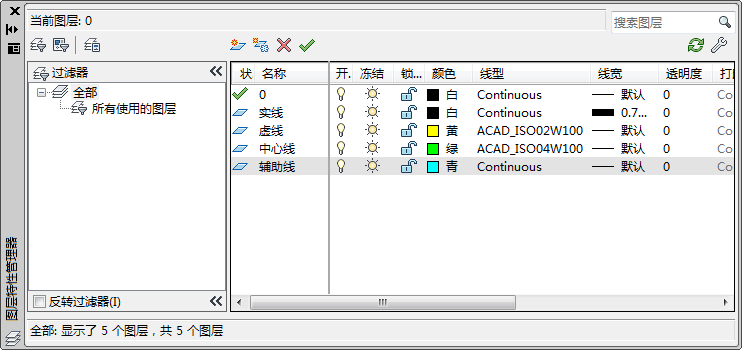
\includegraphics[scale=0.6]{vxingtietuchen.png}
\caption{图层设置}\label{fig:vxintuchen}
\end{figure}

第二步:选择实线图层,使用rectang命令绘制长方体的主视图,如图\ref{fig:cubezhushitu}所示。
\begin{lstlisting}
%命令: RECTANG%
%指定第一个角点或 [倒角(C)/标高(E)/圆角(F)/厚度(T)/宽度(W)]:%
%指定另一个角点或 [面积(A)/尺寸(D)/旋转(R)]: @50,30%
\end{lstlisting}
\begin{figure}[htbp]
\centering
\begin{floatrow}
\ffigbox{\caption{长方体主视图}\label{fig:cubezhushitu}}{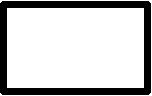
\includegraphics{cubezhushitu.png}}
\ffigbox{\caption{绘制三视图辅助线}\label{fig:cubeaidline}}{
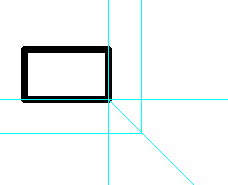
\includegraphics[scale=0.5]{cubeaidline.png}}
\end{floatrow}
\end{figure}

第三步:选择辅助线图层,以主视图的右下点为参照做三视图定位辅助线,如图\ref{fig:cubeaidline}所示。
\begin{lstlisting}
%命令:  XLINE %
%指定点或 [水平(H)/垂直(V)/角度(A)/二等分(B)/偏移(O)]: int%
%于%
%指定通过点:$ @1<0$%
%指定通过点:$@1<90$%
%指定通过点:$ @1<-45$%
%指定通过点:%
%命令: TRIM%
%当前设置:投影=UCS,边=无%
%选择剪切边...%
%选择对象或 $<$全部选择$>$:  找到 1 个%
%选择对象:%
%选择要修剪的对象,或按住 Shift 键选择要延伸的对象,或%
%[栏选(F)/窗交(C)/投影(P)/边(E)/删除(R)/放弃(U)]:%
%选择要修剪的对象,或按住 Shift 键选择要延伸的对象,或%
%[栏选(F)/窗交(C)/投影(P)/边(E)/删除(R)/放弃(U)]:%
%命令: offset%
%当前设置: 删除源=否  图层=源  OFFSETGAPTYPE=0%
%指定偏移距离或 [通过(T)/删除(E)/图层(L)] $<0.0000>$:  20%
%选择要偏移的对象,或 [退出(E)/放弃(U)] $<$退出$>$:%
%指定要偏移的那一侧上的点,或 [退出(E)/多个(M)/放弃(U)]$<$退出$>$:%
%选择要偏移的对象,或 [退出(E)/放弃(U)] $<$退出$>$:%
%指定要偏移的那一侧上的点,或 [退出(E)/多个(M)/放弃(U)] $<$退出$>$:%
%选择要偏移的对象,或 [退出(E)/放弃(U)] $<$退出$>$:%
%命令: trim%
%当前设置:投影=UCS,边=无%
%选择剪切边...%
%选择对象或 $<$全部选择$>$:  找到 1 个%
%选择对象:%
%选择要修剪的对象,或按住 Shift 键选择要延伸的对象,或%
%[栏选(F)/窗交(C)/投影(P)/边(E)/删除(R)/放弃(U)]:%
%选择要修剪的对象,或按住 Shift 键选择要延伸的对象,或%
%[栏选(F)/窗交(C)/投影(P)/边(E)/删除(R)/放弃(U)]:%
%选择要修剪的对象,或按住 Shift 键选择要延伸的对象,或%
%[栏选(F)/窗交(C)/投影(P)/边(E)/删除(R)/放弃(U)]:%
\end{lstlisting}

第四步:以长文体主视图左下点为基准做一条辅助线,以确定俯视图的宽度。然后选择实线图层做出俯视图,如图\ref{fig:cubefushitu}所示。
\begin{lstlisting}
%命令: xline %
%指定点或 [水平(H)/垂直(V)/角度(A)/二等分(B)/偏移(O)]: int%
%于%
%指定通过点: int%
%于%
%指定通过点:%
%命令: rectang%
%指定第一个角点或 [倒角(C)/标高(E)/圆角(F)/厚度(T)/宽度(W)]: int%
%于%
%指定另一个角点或 [面积(A)/尺寸(D)/旋转(R)]: d%
%指定矩形的长度 $<0.0000>$: int%
%于  指定第二点: int%
%于%
%指定矩形的宽度$<0.0000>$: 20%
%指定另一个角点或 [面积(A)/尺寸(D)/旋转(R)]:%
\end{lstlisting}
\begin{figure}[htbp]
\centering
\begin{floatrow}
\ffigbox{\caption{长方体俯视图}\label{fig:cubefushitu}}{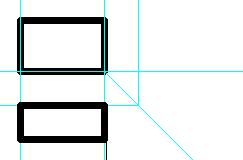
\includegraphics{cubefushitu.png}}
\ffigbox{\caption{长方体三视图}\label{fig:cubethreeview}}{
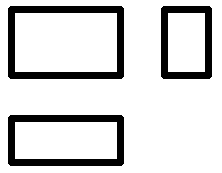
\includegraphics[scale=0.7]{cubethreeview.png}}
\end{floatrow}
\end{figure}

第五步:选择辅助线图层,根据三视图的三等关系做辅助线。然后选择实线图层,完成长方体的三视图,并关闭辅助线图层。最终结果如图\ref{fig:cubethreeview}所示。
\begin{lstlisting}
%命令: xline %
%指定点或 [水平(H)/垂直(V)/角度(A)/二等分(B)/偏移(O)]:%
%指定通过点:%
%指定通过点:%
%命令: xline %
%指定点或 [水平(H)/垂直(V)/角度(A)/二等分(B)/偏移(O)]:%
%指定通过点: per%
%到%
%指定通过点:%
%xline %
%指定点或 [水平(H)/垂直(V)/角度(A)/二等分(B)/偏移(O)]:%
%指定通过点:%
%指定通过点:%
%命令: rectang%
%指定第一个角点或 [倒角(C)/标高(E)/圆角(F)/厚度(T)/宽度(W)]: int%
%于%
%指定另一个角点或 [面积(A)/尺寸(D)/旋转(R)]: int%
%于%
\end{lstlisting}

\subsection{V型块三视图}
我们现在长方体三视图的基础上绘制出V形槽的三视图即完成了V型块的三视图绘制。
第一步:为了方便主视图中的V形槽的绘制,我们先选择中心线图层在主视图中绘制一条中心线,然后再选择实线图层,绘制出V型槽的主视图,结果如图所示。
\begin{lstlisting}
%命令: line 指定第一点: mid%
%于%
%指定下一点或 [放弃(U)]:  $<$正交 开$>$%
%指定下一点或 [放弃(U)]:%
%命令: POINT%
%当前点模式:  PDMODE=0  PDSIZE=0.0000%
%指定点: int 于%
%命令: RECTANG%
%指定第一个角点或 [倒角(C)/标高(E)/圆角(F)/厚度(T)/宽度(W)]:   @20,10%
%指定另一个角点或 [面积(A)/尺寸(D)/旋转(R)]: @10,10%
%命令: POINT%
%当前点模式:  PDMODE=0  PDSIZE=0.0000%
%指定点: int 于%
%命令: line 指定第一点:$ @-15<0$%
%指定下一点或 [放弃(U)]: int%
%于%
%指定下一点或 [放弃(U)]:%
%命令: MIRROR%
%选择对象: 找到 1 个%
%选择对象: % 
%指定镜像线的第一点:%
%指定镜像线的第二点:%
%要删除源对象吗?[是(Y)/否(N)] $<N>$:%
%命令: trim%
%当前设置:投影=UCS,边=无%
%选择剪切边...%
%选择对象或 $<$全部选择$>$:  找到 1 个%
%选择对象: 找到 1 个,总计 2 个%
%选择对象:%
%选择要修剪的对象,或按住 Shift 键选择要延伸的对象,或%
%[栏选(F)/窗交(C)/投影(P)/边(E)/删除(R)/放弃(U)]:  指定对角点:%
%选择要修剪的对象,或按住 Shift 键选择要延伸的对象,或%
%[栏选(F)/窗交(C)/投影(P)/边(E)/删除(R)/放弃(U)]:%
%选择要修剪的对象,或按住 Shift 键选择要延伸的对象,或%
%[栏选(F)/窗交(C)/投影(P)/边(E)/删除(R)/放弃(U)]:%
\end{lstlisting}

第二步:选择辅助线图层,以主视图的V型槽为基础,绘制长对正的辅助线;然后选择实线图层,绘制出V型槽的俯视图,结果如图所示。
\endinput